\documentclass[10pt, openany]{book}
\usepackage{header}
\pgfplotsset{compat=1.18}
\AtBeginDocument{\RenewCommandCopy\qty\SI}

\title{EE Notes}
\author{Damanic Luck}
\date{April 14, 2024}

\begin{document}
% Use this website to find symbols: https://detexify.kirelabs.org/classify.html

% \maketitle

% \setcounter{chapter}{1}
\tableofcontents
\begin{todo}
    \item use this article \href{http://home.iitj.ac.in/~sptiwari/EE314/Lecture2_Semi_Basics_Junction.pdf}{to add to ch1 about doping}
    % \item Chapter 4 diodes
    % \item Chapter 5 mos
    % \item Chapter 6 bjts are optional header
    % \item Chapter 8 integrated circuit amplifiers
    \item practice problems for ch1
    \item practice problems for ch2
    \item finish up ch3 i burned out while trying to be thorough. p117 in reader, p152 in sedra
    \item dead week planning
    \begin{enumerate}
        \item tuesday: finish pn junction, diodes, mosfets
        \item Wedesnday: moscap, amplifiers maybe small signal model
    \end{enumerate}x
\end{todo}

\newpage
\section{Charge Carriers and Doping}

\subsection{Introduction}
We start learning about resistors, capacitors, and inductors from earlier courses such as EECS 16A and 16B. With more components like transistors, diodes, and op-amps (which are all based on semiconductors), we are able to expand upon circuit design. We need to understand semiconductor physics in order to understand how these components operate.
\begin{center}
    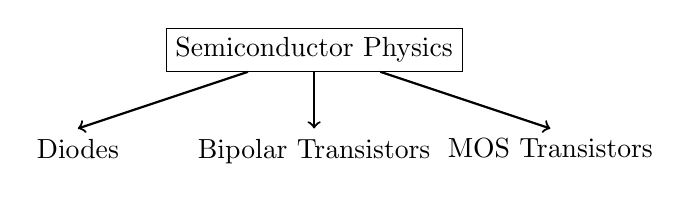
\begin{tikzpicture}
        \node[draw, align=center] (text) {Semiconductor Physics};
        \draw[->, thick] (text) -- ++(0,-1) node[below] {Bipolar Transistors};
        \draw[->, thick] (text) -- ++(-3,-1) node[below] {Diodes};
        \draw[->, thick] (text) -- ++(3,-1) node[below] {MOS Transistors};
    \end{tikzpicture}
\end{center}

We can also redefine Ohm's Law which we know as ($V = IR$) as $J = \sigma \vb{E}$. We can also write resistance($R$) and conductance($G$) in terms of other variables
\begin{gline}
    \item $J$: current density, $A/m^2$ (Amperes per meter squared)
    \item $\sigma$: conductivity, $S/m$ (Siemens per meter)
    \item $\vb{E}$: electric field, $V/m$ (Volts per meter)
\end{gline}

$R = \frac{R}{I} = \rho \frac{l}{A}$ and $G = R^{-1} = \sigma \frac{A}{l}$
\begin{gline}
    \item $\sigma$: conductivity
    \item $\rho$: resistivity
\end{gline}

For collisions in gas, we focus on the idea that initial velocity and direction is lost/randomized after a few collisions. So, when we sum over the random velocities of the particles and average it, it comes out to zero. Average momentum gain is:
\[\bar{\mu} = \frac{\vb{E} q \tau}{M} = \mu \vb{E}, ~~~ \mu := \frac{q \tau}{M} = \frac{\bar{v}}{\vb{E}}\]
\begin{gline}
    \item $\mu$: mobility, $m^2/ (V \cdot s)$
    \item $q$: electric charge, $1.60 \times 10^{-19}$, Coulombs = Amperes/second
    \item $\tau$: mean free time
    \item $M$: mass
    \item $\bar{v}$: average velocity
\end{gline}

Different elements have a different number of outer shell electrons. For semiconductors like silicon, we can increase the temperature to increase its conductivity. Silicon atoms are arranged in a diamond structure and in general, the energy levels that an atom can occupy are discrete. The \textbf{valence band} electrons are at a lower energy state (bound to host atoms) while \textbf{conduction band} electrons are at a higher energy state and are "free" electrons. These electrons are free to move around the crystal and take part in conduction. 

\subsection{Conduction and Fermi Dirac Distribution}
Thermal energy is on average about $\sim 26~eV$ at room temperature How large the \textbf{band-gap}, the gap between the conduction and valence band, determines how conductive a material is:
\begin{itemize}
    \item Insulators: band gap $\sim$ 15 $eV$
    \begin{itemize}
        \item Glass, rubber, oil, plastic, diamond
    \end{itemize}
    \item Semiconductors: band gap $\sim 1 eV$
    \begin{itemize}
        \item Silicon = 1.12 $eV$
    \end{itemize}
    \item Conductors: Not applicable due to overlapping conduction/valence bands
\end{itemize}
Because electrons are a type of particle called a \textbf{fermion}, we can say that 
\[f(\epsilon) = \frac{1}{e^{\frac{E - E_F}{k_B T}} + 1}\]
\begin{gline}
    \item $f(\epsilon)$: occupational probability of a state energy $\epsilon$
    \item $E_F$: fermi energy, $eV$
    \item $k_B$: Boltzmann's constant, $1.380649 \times 10^{-23} J/K$ (Joules per Kelvin)
    \item $T$: temperature in Kelvin
\end{gline}
\subsection{Doping}
\textbf{Doping} is defined as introducing impurities inside a silicon crystal to adjust the number of free electrons that we have. The following materials are commonly used:
\begin{pline}
    \item Group III elements: boron, aluminum, gallium $\rightarrow$ acceptors
    \item Group IV elements: germanium and silicon
    \item Group V elements: phosphorus, arsenic, antimony $\rightarrow$ donors
\end{pline}
Sometimes we assume that the number of electrons we add is much greater than the original free electrons that pure silicon had ($10^{10}$ per cubic centimeter). This leads to the simplification that the number of free electrons in our silicon crystal is $N_D$, where $N_D$ is the number of donor atoms that we add per cubic centimeter.

\subsection{Practice Problems}

\subsection{Sources}
\begin{itemize}
    \item \href{https://www.youtube.com/watch?v=yQDfVJzEymI}{\textcolor{blue}{Razavi Electronics 1, Lec 1, Intro., Charge Carriers, Doping}}
    \item \href{https://file.notion.so/f/f/048d6522-202b-48d4-b5d9-bc005bd602e2/214bf1f0-292f-48d6-9016-737d9f5da155/ee105_reader_v3.pdf?id=237a4300-3dbe-47d1-888b-ffae90d8352b&table=block&spaceId=048d6522-202b-48d4-b5d9-bc005bd602e2&expirationTimestamp=1714435200000&signature=yx-H1qvZJIodPfazOpwXX0Ce2mWMG8skOHl45xoPxus&downloadName=ee105_reader_v3.pdf}{EE105 Reader}
    \item Sedra, Adel S., et al. Microelectronic Circuits. Oxford University Press, 2021
    \item \href{https://eng.libretexts.org/Bookshelves/Materials_Science/TLP_Library_II/22%3A_Introduction_to_Semiconductors/22.2%3A_The_FermiDirac_Distribution}{Engineering LibreTexts: The Fermi-Dirac Distribution}
\end{itemize}



\newpage
\section{Doping and Drift}

\subsection{Sources}
\begin{itemize}
    \item \href{https://www.youtube.com/watch?v=NWolpDgi6_Y}{\textcolor{blue}{Razavi Electronics 1, Lec 2. Doping, Drift}}
\end{itemize}

\newpage
\chapter{PN Junctions}

A \textbf{PN junction} is the junction between an $N$-type semiconductor and $P$-type semiconductor. Understanding the PN junction will set up us for understanding diodes, BJTs, and MOSFETs later. It seems like we draw it as two separate silicon crystals, but in actual practice the $p$ and $n$ regions are part of the same silicon crystal, accomplished by creating regions of different doping.

Plus ("+") signs represent majority holes while minus ("-") signs represent majority el ectrons. The following diagram is from Seda and Adel's \textit{Microelectronic Circuits}.

\begin{figure}[htb]
    \centering
    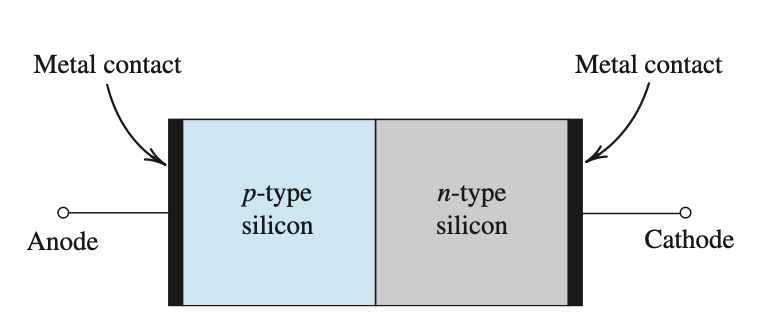
\includegraphics{figs/ch03/pn_junction.png}
    \caption{Simplified physical structure of the PN junction}
\end{figure}

\section{Diffusion Current}
Although it doesn't show it in the diagram, there minority holes generated by thermal ionization in the $n$-type material and there are minority electrons generated in the $p$-type material. Due to concentration difference of holes in the $p$ region and the $n$ region, holes diffuse across the junction from the $p$ side to the $n$ side. This results in \textbf{diffusion current, $I_D$}, whose direction is from the $p$ to $n$ side.

So current Damanic is wondering right now "if this stuff is diffusing then won't this entire block be the same mush at the end." Here we introduce the depletion region. Holes that diffuse across the junction into the $n$ region recombine with majority electrons there. A charge is said to be \textbf{uncovered} when some of the bound positive charge is no longer neutralized by free electrons. This introduces the idea that at a region close to the junction, it is depleted of free electrons and contains unbound positive charge for the $n$ region.

\begin{figure}[htb]
    \centering
    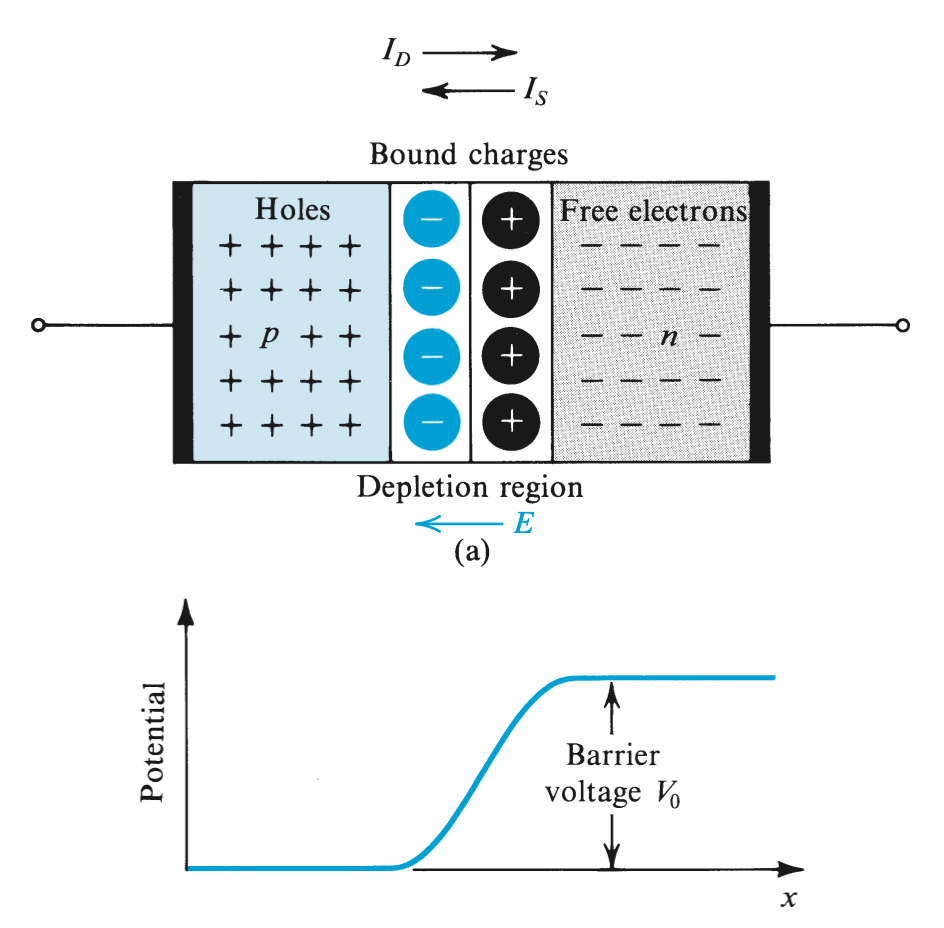
\includegraphics[scale=0.5]{figs/ch03/uncovered_region.png}
    \caption{Top image shows PN-junction with bound charges and bottom image is potential along an axis perpendicular to the junction}
    \label{fig:barrier-voltage1}
\end{figure}

The left side of the PN junction ($p$ region) will be negatively charged while the right side ($n$ region) will be positively charged. To sum it up, this is because at some point, electrons that diffuse across the junction into the $p$ region will recombine with holes, and those holes will disappear leaving uncovered bound negative charge. Vice versa for holes diffusing into the $n$ region. 

From the figure above we see that the $n$ region will be positively charged and the $p$ side if negatively charged. This is the \textbf{depletion region}, or the \textbf{space-charge region} or \textbf{depletion layer}. There are no \textit{mobile} charge carriers present here. Charges on both sides of the depletion region results in an electric field $E$. Here we introduce the idea that a larger barrier voltage results in a small number of carriers that can overcome this barrier. This leads to a decrease in magnitude of diffusion current since it is more difficult for holes to diffuse into the $n$ region and electrons to diffuse into the $p$ region. Referring again to figure \ref{fig:barrier-voltage1}, we see that $V_0$ is the barrier voltage. Therefore the diffusion current $I_D$ has a strong relationship with $V_0$, the voltage drop across the depletion region.

\section{Drift Current and Equilibrium}
Recall that drift current is caused by electric fields and $I_S$ is independent of the value of the depletion-layer voltage $V_0$. Under open-circuit conditions, there is no external current, so 
    \[I_D = I_S\]
This condition is maintained by $V_0$.
\begin{Analysis}{$I_S$ and $I_D$ at Equilibrium}{}
    \begin{gline}
        \item $V_O$: barrier voltage
        \item $I_S$: drift current whose direction is from the $n$ side to the $p$ side of the junction
        \item $I_D$: diffusion current whose direction is from the $p$ side to the $n$ side of the junction
    \end{gline}
    \begin{enumerate}
        \item \textbf{$I_D > I_S$}: more bound charge is uncovered on both sides $\rightarrow$ the depletion layer widens (vertically)$\rightarrow$ $V_0$ increases $\rightarrow$ $I_D$ decreases until $I_D = I_S$ (equilibrium)
        \item \textbf{$I_D < I_S$}: uncovered charge decreases $\rightarrow$ depletion layer narrows (vertically) $\rightarrow$ $V_0$ decreases $\rightarrow$ $I_D$ increases until $I_D = I_S$ (equilibrium)
    \end{enumerate}
\end{Analysis}

Under the zero bias equilibrium condition (no external voltage is applied to the PN junction), does the diffusion and drift current "cancel" out here, meaning that current density is nearly zero. Their individual components are also equal here, i.e. hole/electron drift current is equal to hole/electron diffusion current, respectively.

    \[J_n = 0 = qn_0 \mu_n E_0 + q D_n \frac{dn_0}{dx}\]

$V_0$ has been referred to so far as barrier voltage boltage, but it's also called \textbf{junction built-in voltage}.
    \[\phi_{bi} = V_{th} \ln \left(\frac{N_A N_D}{n_i^2}\right) = \frac{kT}{q} \ln \left(\frac{N_A N_D}{n_i^2}\right)\]
Remember here that $V_th$ is thermal voltage which is $\approx$ 26 mV at room temperature. $\phi_{bi}$ is typically 0.6 V to 0.9V for room temperature silicon. In the EE105 reader, $\phi_{bi}$ and $V_{th}$ has the same meaning as $V_0$ and $V_T$, respectively, in the \textit{Microelectronic Circuits} textbook. I'm writing down the EE105 reader notation here for clarity.

\begin{figure}[htb]
    \centering
    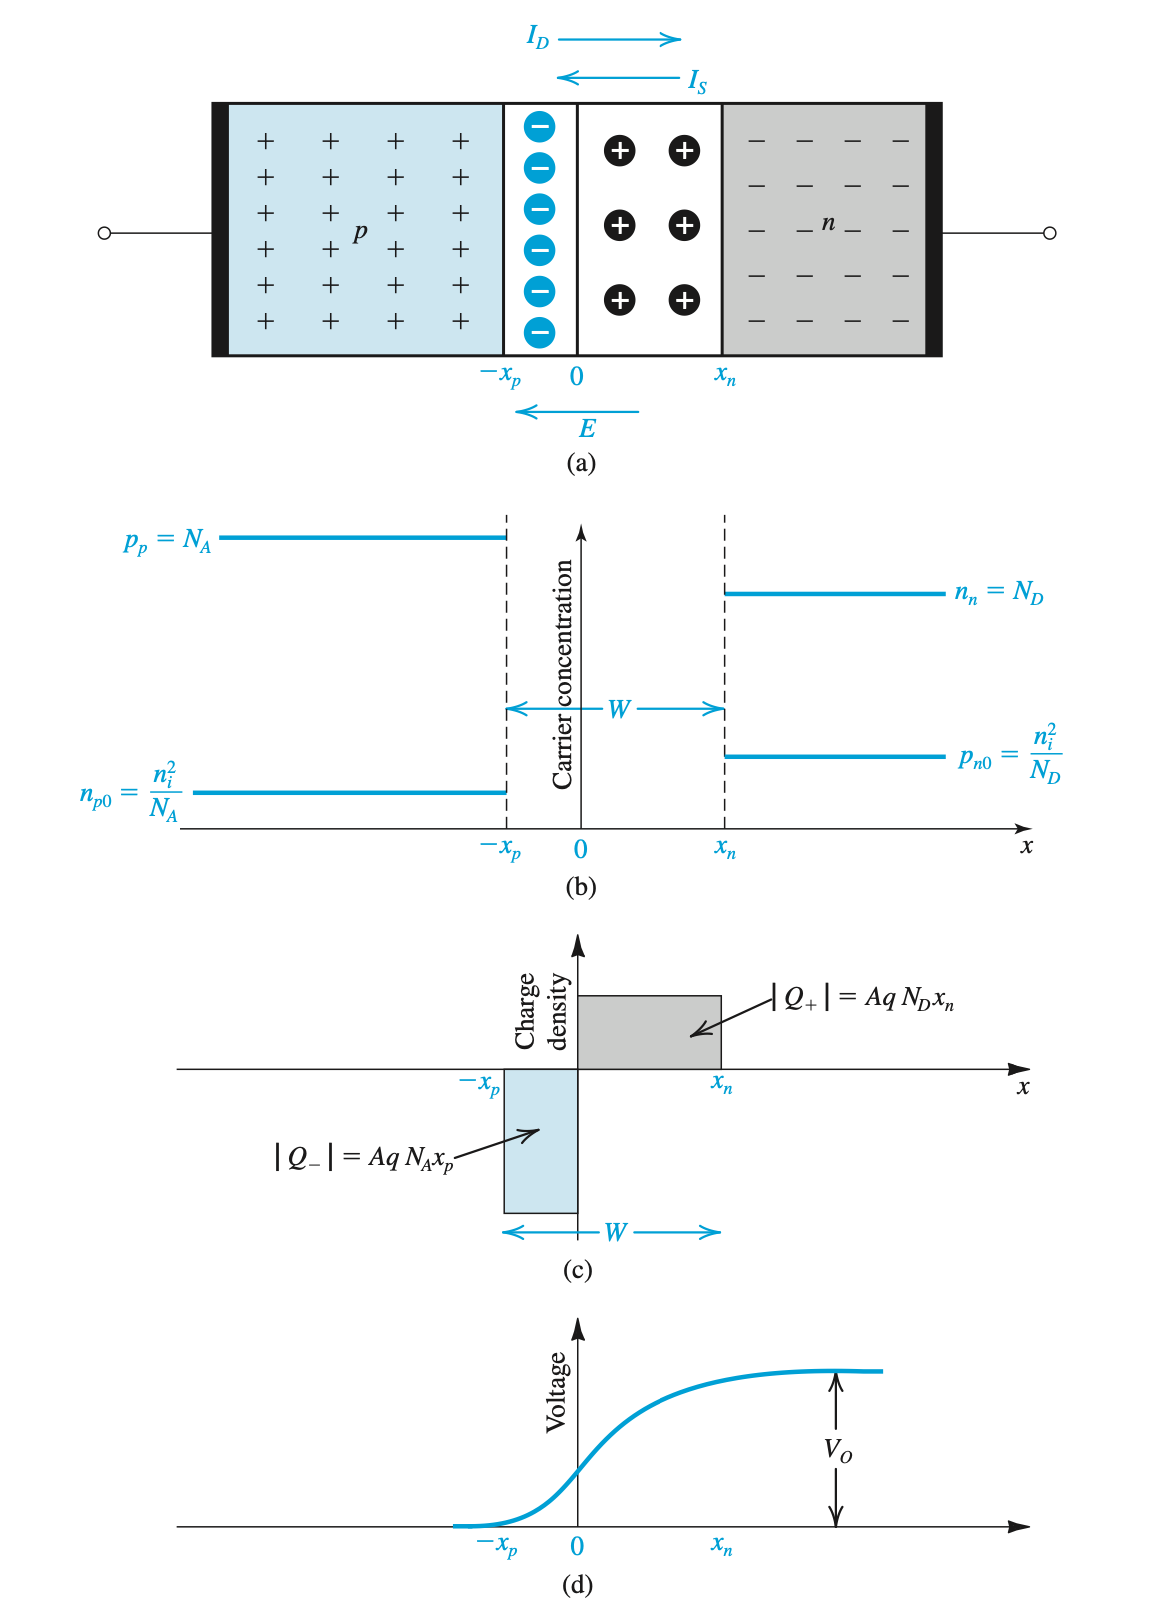
\includegraphics[scale=0.6]{figs/ch03/3_graph.png}
    \caption{Graphs of (a) a PN junction (b) carrier concentrations (c) charge density (d) built in voltage $V_0$}
    \label{fig:3figs}
\end{figure}
\begin{todo}
    \item How we got from each graph
\end{todo}
This graph shows a junction where $N_A > N_D$. If we heavily dope one side, the depletion region will exist almost entirely on the lightly doped side.

\begin{figure}[htb]
    \centering
    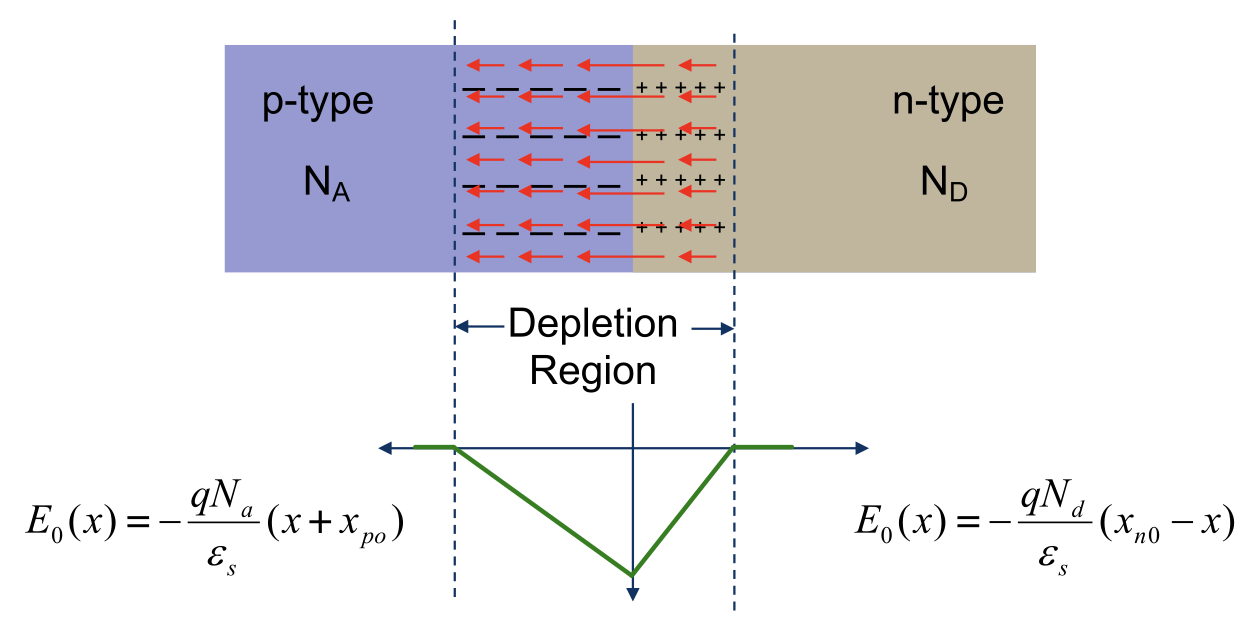
\includegraphics[scale=0.5]{figs/ch03/concentration_reader.png}
    \caption{Graph of electric field of PN junction}
    \label{fig:electric_fields_pn}
\end{figure}

Here in figure \ref{fig:electric_fields_pn}, the electric fields in the depletion region are negative because positive charges are on the right and the negative charges are on the left, assuming zero fields in neutral $P$-region and $N$-regions. Key takeaways due to difference in doping levels in the $N$-type and $P$-type sides:
\begin{pline}
    \item Width of the depletion region is not symmetric
    \item Slope of the electric field is larger in one region than the other
    \item The negative peak of the electric field always occurs at the junction
\end{pline}

\begin{Analysis}{Gauss's Law}{}
    Gauss's Law states that the total electric flux out of a closed surface is equal to the charge enclosed by the permittivity. Electric flux is the electric field multiplied by the area of the surface projected in a plane and perpendicular to the field.
        \[\oint_S {\vec{E_n} \cdot \vec{d}s = \frac{1}{{\varepsilon _0 }}} Q_{inside}\]
    \begin{todo}
        \item finish this
    \end{todo}
    By Gauss's Law, the total fixed charged in the $N$-region is the same as the total fixed charge in the $P$-region.
        \[q N_A x_{p0} = q N_D x_{n0}\]
\end{Analysis}
Here we'll derive the equations for depletion width, which are dependent on externally applied voltage, which are given by the following. The zero is for the zero bias case.
\begin{itemize}
   \item[] Depletion width on N-side: {\Large $x_{n_0} = \sqrt{\frac{2 \epsilon_s \phi_{bi}}{q N_D} (\frac{N_A}{N_A + N_D})}$}
   \item[] Depletion width on P-side: {\Large $x_{p_0} = \sqrt{\frac{2 \epsilon_s \phi_{bi}}{q N_A} (\frac{N_D}{N_A + N_D})}$}
   \item[] Built in potential: {\Large $\phi_{bi} \equiv \phi_n = \phi_p > 0$}
   \item[] Total depletion width {\Large $X_{dep_0} = x_{n_0} + x_{p_0} = \sqrt{\frac{2 \epsilon_s \phi_{bi}}{q}(\frac{1}{N_A} + \frac{1}{N_D})}$}
\end{itemize}

\begin{todo}
    \item derivation here
\end{todo}
For the zero bias case (under thermal equilibrium), net current is zero. Diffusion current is very small since few carriers have enough energy to penetrate the barrier. Drift current is small since minority carriers are few.
\section{Reverse Bias}
\begin{figure}[H]
    \centering
    \begin{circuitikz}
        \draw (0,0) to [battery2, l=$V_D < 0$ , invert] (0,2)
        to [short] (2,2)
        to [full diode, v^=$-\phi_{bi}+V_D$,] (2,0)
        to (0,0);
    \end{circuitikz}
    \label{fig:reverse_bias}
\end{figure}

The above section was discussing the PN junction at equilibrium. At equilibrium, the $PN$-junction doesn't draw any current. Under reverse bias like in figure above, meaning that a negative voltage is applied, charge will increase and the depletion region widens horizontally. We can rewrite the depletion width formulas from above as a function of $V_D$.
\begin{itemize}
    \item[] {\Large $x_n(V_D) = \sqrt{\frac{2 \epsilon_s (\phi_{bi} - V_D)}{q N_D} (\frac{N_A}{N_A + N_D})} = x_{n_0} \sqrt{1 - \frac{V_D}{\phi_{bi}}}$}
    
    \item[] {\Large $x_p(V_D) = \sqrt{\frac{2 \epsilon_s (\phi_{bi} - V_D)}{q N_A} (\frac{N_D}{N_A + N_D})} = x_{p_0} \sqrt{1 - \frac{V_D}{\phi_{bi}}}$}

    \item[] {\Large $X_{dep_0} = x_n(V_D) + x_n(V_D) = \sqrt{\frac{2 \epsilon_s (\phi_{bi} - V_D)}{q}(\frac{1}{N_A} + \frac{1}{N_D})} = X_{dep_0} \sqrt{1 - \frac{V_D}{\phi_{bi}}}$}
\end{itemize}
Keep these in mind: 
\begin{pline}
    \item Minority drift current is independent of the barrier height ($\phi_{bi}$)
    \item Diffusion current is a strong exponential function of the barrier height
\end{pline}

\section{Forward Bias}
This occurs when $V_D$ is nonnegative. A forward bias results in a exponential increase in the number of carriers, which have enough energy to break the barrier. This results in an exponential increase in diffusion current. Drift current doesn't change with forward bias. 

\begin{todo}
    \item skipped small signal model for this
    \item skipped a lot of practice problems for this too
\end{todo}

\section{Practice Problems}
\begin{enumerate}
    \item Show that 
        \[V_0 = \frac12 (\frac{q}{\epsilon_s})(\frac{N_A N_D}{N_A + N_D}) W^2\]
    % \begin{Ans}
    %     We know that $\phi_{bi} = V_{th} \ln \left(\frac{N_A N_D}{n_i^2}\right) = \frac{kT}{q} \ln \left(\frac{N_A N_D}{n_i^2}\right)$
    % \end{Ans}
    \item Show that for a PN junction in which the $p$ side is much more heavily dped than the $n$ side (i.e. $N_A \gg N_D$) referred to as a $p^+ n$ diode. The following can be written as follows:
        \begin{align*}
            W &\simeq \sqrt{\frac{2 \epsilon_s}{q N_D}V_0}, ~~~~~ x_n \simeq W, ~~~~~ x_p \simeq \frac{W}{N_A / N_D} \\
            Q_j &\simeq A q N_D W, ~~~~~ Q_j \simeq A \sqrt{2 \epsilon_s q N_D V_0}
        \end{align*}
    
    \item For a Si PN junction that looks like this, where $N_A = 1 \times 10^{18}$ \conc and $N_D = 1 \times 10^{17}$ \conc. Given the built-in potential is 0. V and the relatively permittivity of Si is 12. No voltage is applied.
    \begin{figure}[H]
        \centering
        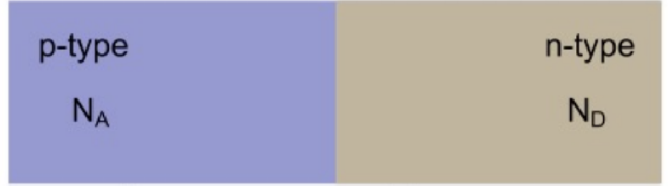
\includegraphics[scale=0.5]{figs/ch03/ans2.png}
    \end{figure}
    \begin{enumerate}
        \item Draw the charge along the horizontal axis.
        \item Draw the electric field along the horizontal axis. Label the critical points such as charge density, depletion width, and maximum electric field in your graphs.
    \end{enumerate}

    \item Considering a PN junction where the $n$ side is doped with $N_D = 10^{17}$ \conc and $p$ side is doped with $N_A = 10^{20}$ \conc, $n_i = 10^{10}$ \conc, kT/q = 26 mV, $\mu$n = 100 \mobility at $p$ side, $\mu$p = 400 \mobility at n side, L$_n$ = 2.3 \mun at $p$ side, and L$_p$ = 3.2 \mun at $n$ side, vacumn permittivity is $\epsilon_0 = 8.854 \times 10^{-12}$ C\sq/ (N $\cdot$ m\sq), the permittivity of silicon is 11.7$\epsilon_0$. Area of the PN junction is 1 \mun\sq
    \begin{enumerate}
        \item Calculate the built-in potential.
        \item Calculate the total depletion width at zero bias.
        \item Draw the electric field profile at zero bias (You need to calculate the maximum electric field). The left-hand side is N and the right-hand side is P.
        \item Calculate the depletion capacitance when the bias -1V. 
        \item Calculate the current when the bias is 1V.
        \item Find out the small-signal resistance and diffusion capacitance at 1V Given $\tau = 1 \mu$s. 
    \end{enumerate}
\end{enumerate}

\section{Sources}
\begin{itemize}
    \item Sedra, Adel S., et al. Microelectronic Circuits. Oxford University Press, 2021: Specifically screenshots of the graphs I need to redo this when I learn how to use graphing/tikzpicture better in LaTex
    \item \href{https://file.notion.so/f/f/048d6522-202b-48d4-b5d9-bc005bd602e2/214bf1f0-292f-48d6-9016-737d9f5da155/ee105_reader_v3.pdf?id=237a4300-3dbe-47d1-888b-ffae90d8352b&table=block&spaceId=048d6522-202b-48d4-b5d9-bc005bd602e2&expirationTimestamp=1714435200000&signature=yx-H1qvZJIodPfazOpwXX0Ce2mWMG8skOHl45xoPxus&downloadName=ee105_reader_v3.pdf}{EE105 Reader}
    \item Q1 and Q2 are excercises from Sedra, Adel chapter3
    \item Q3 from here is Q4 from EE105 HW6
    \item Q4 from here is Q1 from EE105 Hw7
    \item \href{https://byjus.com/jee/gauss-law/}{Explanation of Gauss's Law}
\end{itemize}
\end{document}